\section{Digitale Uebermittlung analoger Signale \schaum{90}}

%\subsection{PCM - Pulse Code Modulation}
\begin{center}
	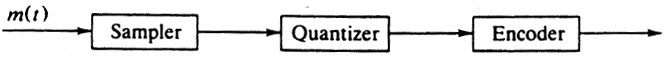
\includegraphics[width=10cm]{bilder/dig_pcm_blockdiagramm.png}
\end{center}
\begin{enumerate}
  \item Abtastung (Sampler): Zeitdiskretisierung 
  \item Quantisierung (Quantizer): Amplitudendiskretisierung
  \item Encoder (Codierung)
\end{enumerate}

Einige Vorteile der Digitalisierung: bis 100\% Störungsfrei, Algorithmen
einfach auf Signal anwendbar, Verschlüsselung leicht gemacht.

\subsection{Bandbeschränkung}
	Damit das Signal mit einer endlichen Abtastrate erfasst werden kann, muss es bandbeschr\"ankt sein.\\
	F\"ur ideal band-beschränktes Basisbandsignal $m(t)$ gilt: $|M(\omega)| = 0$ für $|\omega| > 2\pi B_m$ 
\subsubsection{Aliasing}
	Bei nicht-bandbeschränkten Signalen treten bei der Abtastung \textit{zwingend} Aliasing-("Falschsignal-") Effekte auf.

\subsection{Abtastung (Sampling) \schaum{91}}
	Ein ideale Abtastung besteht theoretisch aus einer periodischen Abfolge von Dirac-Pulsen
	$\delta_{T_S}$ mit dem Abstand $T_s = \frac{1}{f_s}$. Dieses Spektrum erhält man mittels der Fourier-Reihe. \\ \\
	%$$ c_n = \frac{1}{T} \int\limits_{-T/2}^{T/2} \delta_{T_S}(t) e^{-j n \omega n t} dt = 
	%\frac{1}{T} \quad \Rightarrow \quad X(j \omega) = \sum\limits_{n = -\infty}^{+\infty} c_n
	%\delta(\omega - n \omega_0) \qquad 
	\textbf{Idealer Sampler:}
	$$\delta_{T_S}(t) = \sum\limits_{n=-\infty}^{+\infty} \delta(t-nT_S) \; \laplace \; \omega_S \cdot \delta_{\omega_S} (\omega) = \omega_S \sum\limits_{n=-\infty}^{+\infty} \delta(\omega - n \omega_S) \qquad \text{mit  } \omega_S = \frac{2\pi}{T_S}$$
	\begin{center}
		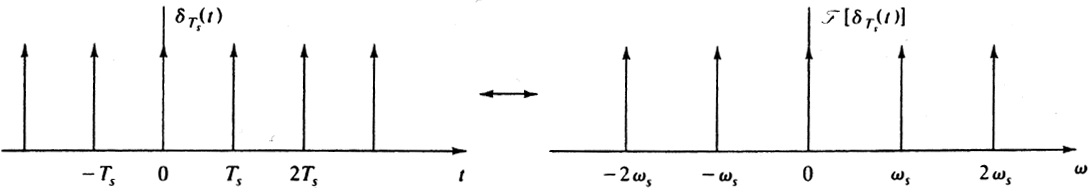
\includegraphics[width=10cm]{bilder/dig_sampler_ideal.png}
	\end{center}

	\textbf{Idealer Abtaster:}
	\begin{equation*}
		 m_s(t) = m_s(t) \cdot \delta_{T_s} = \sum_{n=-\infty}^{+\infty} m(nT_s) \cdot \delta(t-nT_s) \quad \laplace \quad
		M(\omega) = \frac{1}{2\pi}M(\omega)\ast (\omega_s\cdot\delta_{w_s}(\omega)) = \frac{1}{T_s} \sum_{n=-\infty}^{+\infty}M(\omega-n\omega_s)
	\end{equation*}
	\begin{center}
			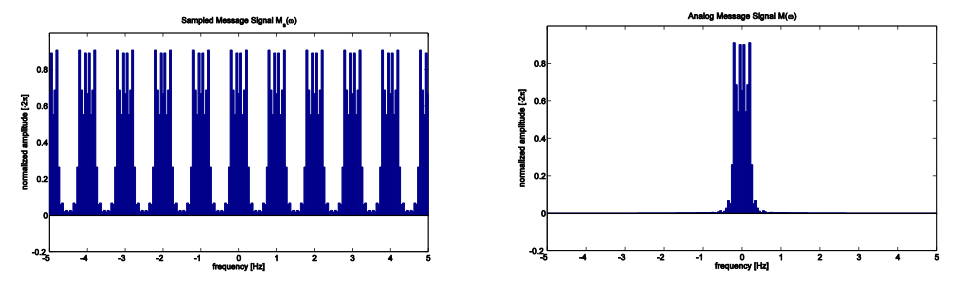
\includegraphics[width=10cm]{bilder/dig_abtaster_ideal_spektrum.png}
		\end{center}
\subsection{Rekunstruktion von $m(t)$ aus $m_s(t)$}
Falls das Abtasttheorem bei der Abtastung erf\"ullt war, kann das Basisbandsignal $m(t)$ durch ein Tiefpassfilter mit Eckfrequenz $\omega_c = \frac{\omega_s}{2} = \frac{\pi}{T_s} $ und Verst\"arkungsfaktor $K=T_s$ rekonstruiert werden.  

\begin{equation*}
	m(t) = \left({\sum_{n=-\infty}^{+\infty}m(nT_s)\cdot\delta(t-nT_s)\ast\frac{\sin(\omega_ct)}{\omega_ct}}\right) = 
	\sum_{n=-\infty}^{+\infty}m(nT_s)\cdot\frac{\sin(\omega_c(t-nT_s))}{\omega_c(t-nT_s)}
\end{equation*}
Dies entspricht einer Folge von gewichteten $\sinc$-Funktionen an den Stellen $nT_s$.

\subsubsection{Abtasttheorem - Nyquist Theorem}
Ein Nachrichtensignal muss mind. mit dem Doppelten seiner Eigenfrequenz abgetastet werden. \\
Ansonsten können sich die Signale im Spektralbereich \text{\"uberlappen}.  
%Um dies zu verhindern wird ein sogenannter \textbf{Anti-Aliasing Filter} der Abtastung vorgeschaltet.
\\ \\
\textbf{Bei Basisbandabtastung:}\\
\hspace*{3cm}
\begin{minipage}[t][2.0cm][c]{8cm}
	$ f_s > 2 f_m  = f_N$ \\
	$ f_N = 2 \cdot B_m $ \\
	$ f_{Nyq} = \frac{f_s}{2}$ \\
	$ T_N = \frac{1}{2\cdot B_m} = \frac{1}{f_N} $
\end{minipage}
\begin{minipage}[t][2.5cm][c]{10cm}
	$f_s$ Samplingfrequenz, $[f_s] = Hz$ \\
	$f_m$ Nachrichtenfrequenz, $[f_m] = Hz$ \\
	$B_m$ Nachrichtenbandbreite, $[B_m] = Hz$ \\
	$f_N$ Nyquistrate, $[f_N] = Hz$ \\
	$f_{Nyq}$ Nyquistfrequenz, $[f_{Nyq}] = Hz$ \\
	$T_N$ Nyquistintervall, $[T_N] = s$ \\	
\end{minipage}

\subsubsection{Subsampling/Bandpassabtastung}
Handelt es sich bei dem Nachrichtensignal um ein \textbf{Bandpasssignal}, so kann mit einer noch
kleiner Samplingfrequenz abgetastet werden, dies nennt man \textbf{Subsampling}. \\
Vorgehen: 1. Alle möglichen $n$ bestimmen (ganzzahlig). 2. Alle möglichen Frequenzintervalle für
$f_s$ bestimmen.

\begin{minipage}[t][2.2cm][c]{8cm}
$$ 1 \leq n \leq \frac{f_u}{f_u - f_l} $$
$$ \frac{2 \cdot f_u}{n} \leq f_s \leq \frac{2 \cdot f_l}{n-1}$$
\end{minipage}
\begin{minipage}[t][2.2cm][c]{9cm}
	$f_s$ Samplingfrequenz, $[f_s] = Hz$ \\
	$f_l$ Minimale (lower) Nachrichtenfrequenz, $[f_l] = Hz$ \\
	$f_u$ Maximale (upper) Nachrichtenfrequenz, $[f_u] = Hz$ \\
	$n$ Subsampling-Faktor, \textcolor{red}{ganzzahlig} \\
	$n \geq 2$ sonst kein Subsampling möglich \\
\end{minipage}

\subsubsection{Oversampling}
Ein weiterer Begriff bezüglich Sampling ist das \textbf{Oversampling}, welches bei \textbf{DAC}s
(Digital-Analog Converter) angewendet wird. \\
	\begin{minipage}{9cm}
		Hierbei \textbf{interpoliert} ein DSP zusätzliche Samples, um die Sample-Rate der D/A-Wandlung zu erhöhen.\\
		Folgende Vorteile resultieren daraus:\\ 
		- \textbf{Originalgetreueres} Nachrichtensignal \\
		- Aperture Effekt wird kleiner\\
		- kleinere \textbf{Filtersteilheit} notwendig.\\
		- verbessert SNR
		
	\end{minipage}
	\begin{minipage}{10cm}
		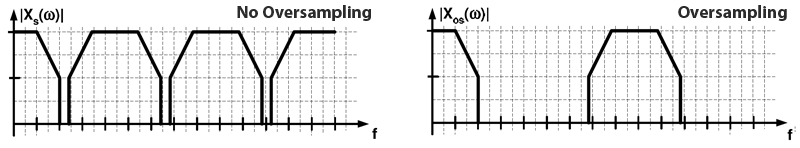
\includegraphics[width=10cm]{bilder/dig_oversampling.png}
	\end{minipage}

\subsubsection{Natural Sampling \schaum{111-5.9}}
Signal mit Periodendauer $T_S$ wird für die Zeit $d$ geschlossen. Amplitude ist bleibt
während Sample nicht konstant. Bei dieser Sampling-Art besteht \textbf{kein Aperture-Effekt}\\

	\begin{minipage}{18cm}
		\begin{equation*}
			m_{ns} = m(t)\cdot\frac{1}{d}rect_{T_s}(t/d) \qquad \text{mit} \quad rect_{T_s}(t/d) = \sum_{n=-\infty}^{+\infty}rect((t-nT_s)/d)\qquad \text{mit} \quad rect(t/d) = \begin{cases}
				1 & |t| < d/2\\
				0 & |t| > d/2
			\end{cases}
		\end{equation*}
	\end{minipage}
	
	\begin{minipage}{12cm}
		\begin{equation*}
			M_{ns} = \sum_{n=-\infty}^{+\infty}c_n \cdot M(\omega-n\omega s) \quad \text{mit $c_n$ von Rechteckimpuls}
		\end{equation*}
		\begin{equation*}
			c_n = \frac{d\cdot A}{T_s}\frac{\sin(n\omega_s d/2)}{n \omega_s d/2}
		\end{equation*}
	\end{minipage}
	\begin{minipage}{5cm}
			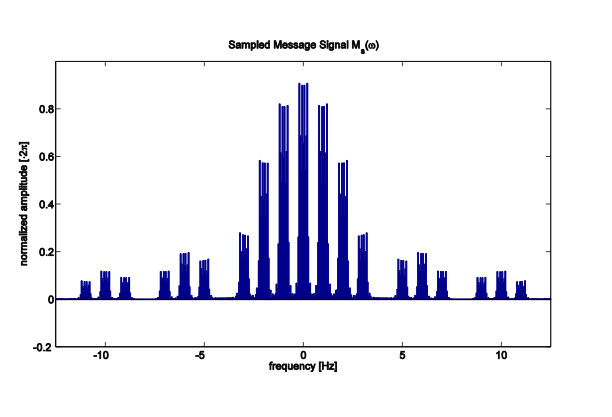
\includegraphics[width=5cm]{bilder/dig_naturalsampling_spektrum}
	\end{minipage}\\
	\begin{center}
		\begin{minipage}{12cm}
				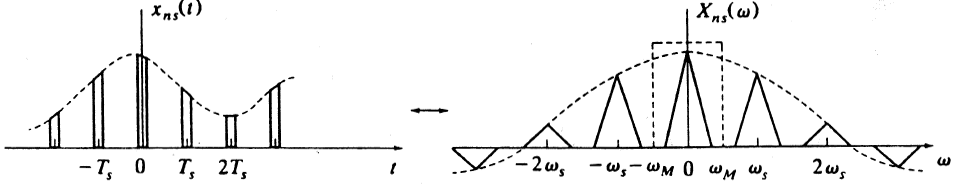
\includegraphics[width=12cm]{bilder/dig_naturalsampling.png}
			\end{minipage}
	\end{center}
\newpage

\subsubsection{Flat-Top Sampling - Sample \& Hold \schaum{112-5.10}}
Das Sample hat die Breite $d$ und bleibt über diese Zeit konstant. \\
Anwendungsbeispiel: A/D-Wandler, Sample \& Hold Schaltung. \\
	\begin{equation*}
		m_{_{FT}}(t) = \overbrace{\left( \sum_{n=-\infty}^{+\infty} m(nT_s) \cdot \delta(t-nT_s)\right)}^{m_s(t)} \ast rect(t/d)
		\quad \laplace \quad
		M_{FT}(\omega) =\left(\frac{1}{T_s} \sum_{n=-\infty}^{+\infty} M(\omega -n\omega_s)\cdot d \frac{\sin(\omega \cdot d/2)}{\omega\cdot d/2}\right)
	\end{equation*}
	\begin{center}
		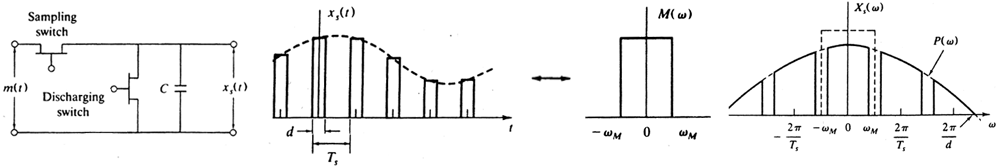
\includegraphics[width=17.5cm]{bilder/dig_flattopsampling.png}
	\end{center}
Das Spektrum des gesampelten Signals wird bei \textbf{höheren Frequenzen} gedämpft, dieses Phänomen
wird als \textbf{Aperture Effect} bezeichnet. Dies kann mit entsprechenden Filtern, oder Vorkompensation 
korrigiert werden.\\
%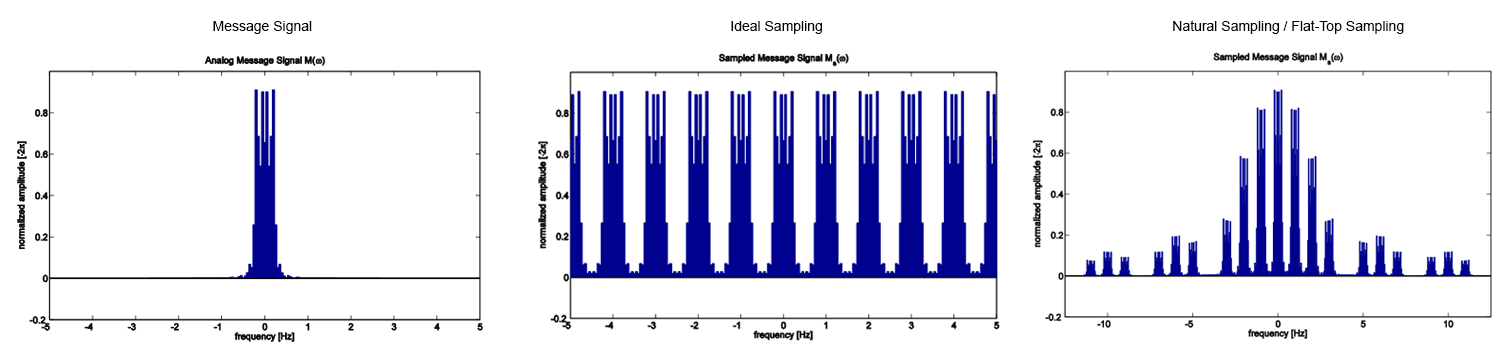
\includegraphics[width=17.5cm]{bilder/dig_sampling_spec.png}
\\

\subsection{Quantisierung (Quantizing)\schaum{93-5.6}}
	\begin{center}	
		\textbf{Gleichförmig} \hspace{3cm}
		\textbf{Ungelichgörmig} \hspace{2.9cm}
		\textbf{$\mu$-Law} \hspace{3cm}
		\textbf{A-Law}  \\
		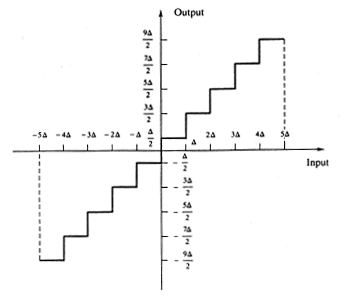
\includegraphics[height=4cm]{bilder/dig_quant_gleichfoermig.png} \hspace{0.5cm}
		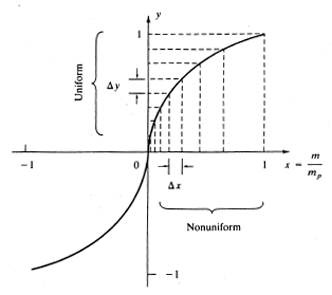
\includegraphics[height=4cm]{bilder/dig_quant_ungleichfoermig.png} \hspace{0.5cm}
		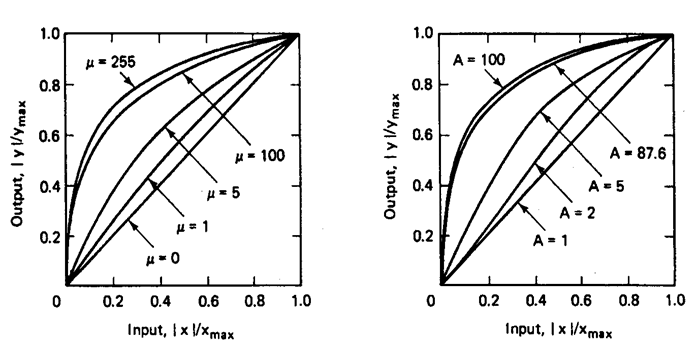
\includegraphics[height=4cm]{bilder/dig_quant_lulaw_ralaw.png}	
	\end{center}
	$\mu$-Law und A-Law sind vor allem bei Signalen mit hohem Crest-Faktor von
	Vorteil: $C = \frac{\left|x\right|_{pk}}{x_{RMS}} =
	\frac{\left|x\right|_{pk}}{\sqrt{x_{Leistung}}}$
\renewcommand{\arraystretch}{1}

\subsubsection{Gleichförmige(Uniform) Quantisierung}
\begin{multicols}{2}
	$ \Delta = \frac{m_{pk}}{2^{n-1}} = \frac{2 \cdot m_{pk}}{L} \qquad \qquad L =
	2^n$\\
	$q_e \leq |\frac{\Delta}{2}|$\\
	$ N_q = \left< q_e^2 \right> = \frac{\Delta^2}{12} =
	\frac{m_{pk}^2}{L^2 \cdot 3}$ \\
	$ S = \left( \frac{ m_{pk} }{C} \right)^2$ \\
	$ \text{SNR}_{q} =\frac{S}{N_q}=\frac{m_{pk}^2}{q_e^2C^2} = \frac{12\cdot m_{pk}^2}{\Delta^2\cdot C^2}$\\
	$\text{SNR}_{q} \left[dB\right] =10 \log(\text{SNR}) \cdot dB \approx n \cdot
	6.02dB$ \\ \\
	
		$\text{SNR}_{q}=n*6.02+10*\log(\dfrac{3}{C^{2}})dB$\\\\
	\textbf{S nach TP-Filter:}\\
	$S_{TP} = \sum\limits_{n=-k}^{k} |c_n|^2 $
\columnbreak

	\begin{tabular}{l l}
		$\Delta$ & Intervallbreite \\
		$L$ & Anzahl Intervalle \\
		$n$ & Wortlänge der Samples, [Anzahl Bit] \\
		$m_{pk}$ & Amplitude des Nachrichtensignals \\
		$C$ & Crestfaktor des Nachrichtensignals \\
		$q_e$ & Quantisierungsfehler \\
		$<q_e^2>$ & Quantisierungsrauschen \\
		$S$ & Signalleistung\\
		$\text{SNR}_{q}$ & Signal-to-Noise Ratio, $[\text{SNR}] = dB$ \\
		$k$ & Anzahl durchgelassene Harmonische
	\end{tabular}
\end{multicols}

\newpage
\subsubsection{Ungleichförmige(Nonuniform) Quantisierung \schaum{95-9.5C}}
Bei tiefen Nutzsignalen hat die gleichförmige Quantisierung den Nachteil einer schlechten SNR
(Signal - Geräusch Abstand). \\
Beihilfe schafft die Ungleichförmige Quantisierung z.B. bei Telefonie
A-Law-(Europa) oder $\mu$-Law-Codierung (USA, Japan)). \\
Praktisch wird dies mit einem sogenannten \textbf{Kompressor} und einem nachgeschalteten
gleichförmigen Quantisierer realsiert.

\begin{minipage}{9cm}
\[ y_{\mu-Law}(x) = \sgn(m) \frac{\ln(1+\mu\cdot|x|)}{\ln(1+\mu)} \qquad \text{mit} \quad
x = \frac{m}{m_{pk}}\]
\vspace*{-0.5cm}
\begin{align*}\text{SNR}_{\mu-Law} &\approx 10 \log \dfrac{3 L^2}{[\ln(1 + \mu)]^2} \\
	&\approx -10.1 + 6.02 \cdot n \: dB \quad \text{f\"ur} \; \mu = 255 
\end{align*}
	\[ \Delta y_{min_{\mu-Law}} \text{bei 8 bit} = \frac{1}{127}
	\]
	
\end{minipage}
\begin{minipage}{9cm}
\[y_{A-Law}(x)=\begin{cases} \frac{A}{1+ \ln A} x & \mbox{wenn } |x| \le \frac{1}{A} \\
	\frac{1 + \ln A\cdot |x|}{1+ \ln A}\sgn(m) & \mbox{wenn } \frac{1}{A} < |x| \le 1 \end{cases} \]
\[\text{SNR}_{A-Law} \approx 10 \log \dfrac{3 L^2}{(1+\ln A)^2}\]

	\[ \Delta y_{min_{A-Law}} \text{bei 8 bit} = \frac{1}{128}
		\]
\end{minipage}

\subsection{Codierung (Encoding) \schaum{96-5.8}}

\subsubsection{PCM-Signale}
\begin{minipage}{9cm}
	\[f_s > 2 \cdot B_m  \qquad \qquad n = \log_2L\]  
	\[R_B = f_s \cdot n > 2 \cdot n \cdot B_m\] 
	\[B_{eff} > B_{PCM} = \frac{1}{2} n \cdot f_s > n \cdot B_m\]
	SNR für vollausgesteuerten Sinus ($C = \sqrt{2}$):	
	\[(SNR)_0 = \frac{3}{2}L^2\]
	\[(SNR)_{0dB}
		= 1.76dB + n \cdot  6.02dB\]
\end{minipage}
\begin{minipage}{9cm}
	$f_s$ Samplingrate, $[f_s] = Hz$ \\
	$n$ Bits pro Sample, \textcolor{red}{ganzzahlig} \\
	$R_B$ Bitrate des PCM-Signals, $[R_B] = \frac{bit}{s}$ \\
	$B_m$ Signalbandbreite, $[B_m] = Hz $ \\
	$B_{PCM}$ Bandbreite PCM Signal, $[B_{PCM}] = Hz $\\
	$T_B$ Bitdauer = $\frac{1}{R_B}$
\end{minipage}


\subsubsection{Delta Modulation \schaum{97-5.9}}
\begin{minipage}{6cm}
	Mit Summierer\\
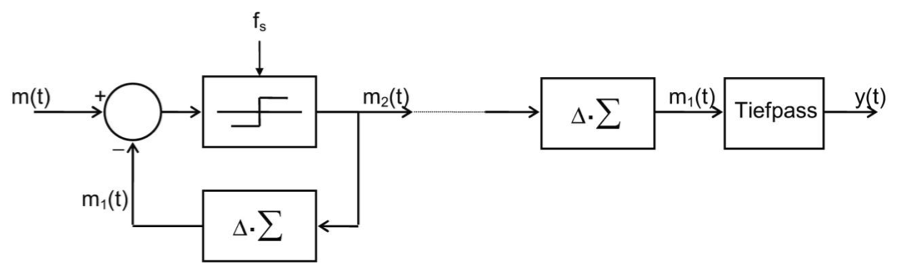
\includegraphics[width = 6cm]{bilder/dig_delta_modulator_schema_sum}
\end{minipage}
\hspace{0.5cm}
\begin{minipage}{6cm}
	Mit Integrierer\\
	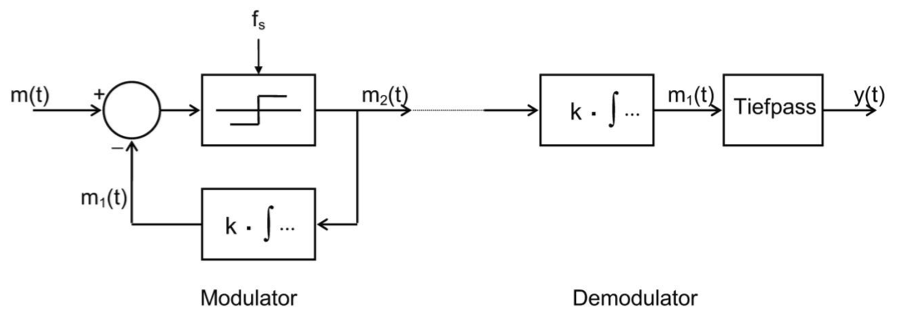
\includegraphics[width = 6cm] {bilder/dig_delta_modulator_schema_int}
\end{minipage}
\hspace{0.5cm}
\begin{minipage}{4cm}
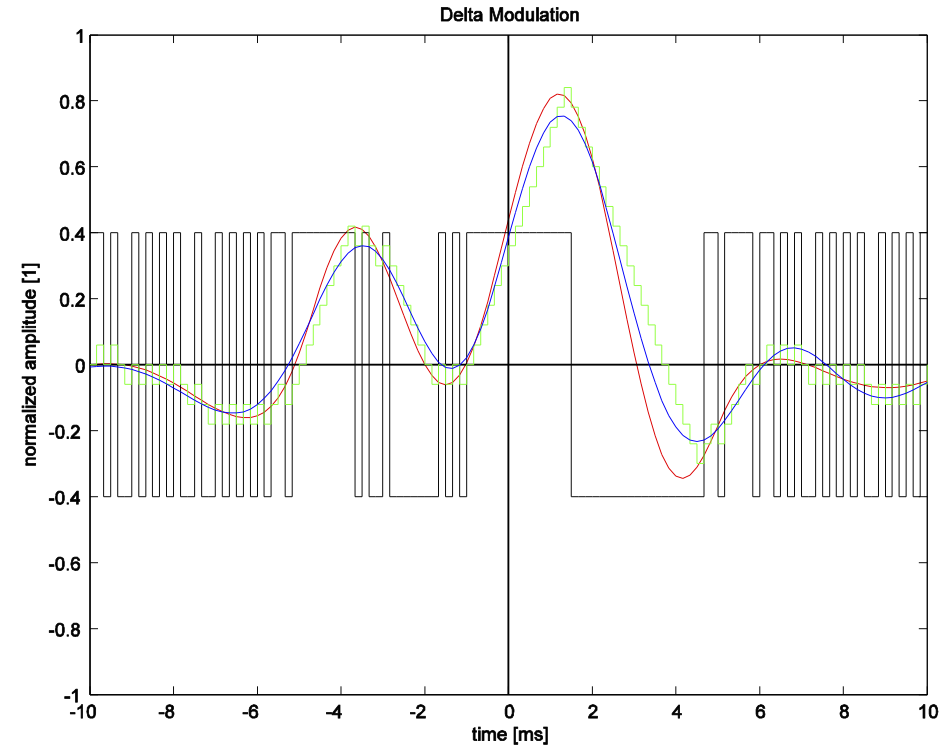
\includegraphics[width = 4cm] {bilder/dig_delta_modulation}
\end{minipage}

\begin{minipage}{9cm}
	\[\frac{\Delta}{T_s} = \Delta \cdot f_s > \left| \frac{d m(t)}{dt} \right|_{max}\]
	\[(\text{SNR})_{0dB} = 10 \cdot \log\left(\frac{1}{2}\frac{3 f_s^3}{8 \pi^2 f_m^2 f_M}\right) dB\]
	\[N_q = <q_e^2> = \frac{\Delta^2}{3}\] 
\end{minipage}
\begin{minipage}{9cm}
	$f_s$ Samplingrate, $[f_s] = Hz$ \\
	$f_m$ Signalfrequenz, $[f_m] = Hz$ \\
	$f_M$ Grenzfrequenz des TP-Filters, $[f_M] = Hz$ \\
	$ \quad \text{Dabei gilt: }f_M \geqq f_m \quad \& \quad f_M \ll f_s$
	$B_m$ Signalbandbreite, $[B_m] = Hz $ \\
	$B_{PCM}$ Bandbreite PCM Signal, $[B_{PCM}] = Hz $\\
	$\Delta$ Schritthöhe\\
	$<q_e^2>$ Quantisierungsrauschen \\
\end{minipage}

\subsubsection{Delta-Sigma Modulation}
\begin{minipage}{10cm}
	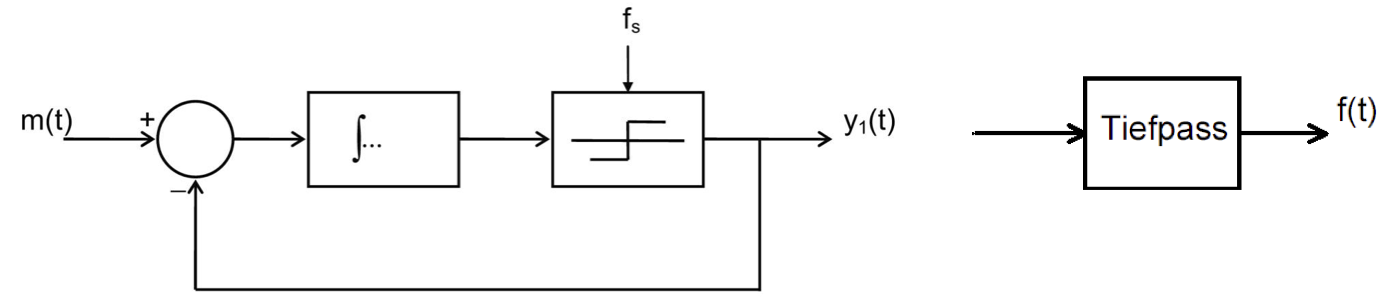
\includegraphics[width=10cm]{bilder/dig_delta_sigma_modulator_schema}
\end{minipage}
\begin{minipage}{6cm}
	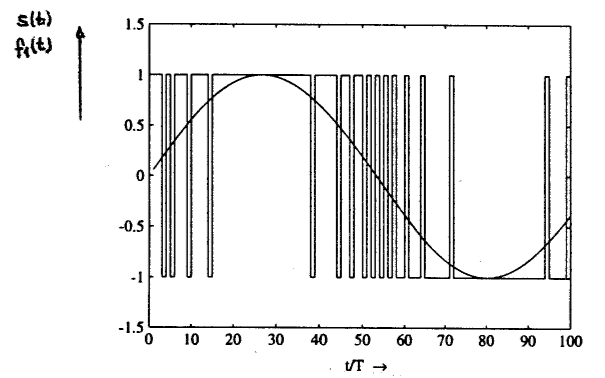
\includegraphics[width=6cm]{bilder/dig_delta_sigma_modulation}
\end{minipage}
	

\newpage
\subsubsection{Leitungscodierung \schaum{99-5.10}}
Je nach Anforderungen (DC-Freie Übertragung, Clock-Rückgewinnung, Störfestigkeit,
Bandbreitenbedarf, Erkennung von Übertragungsfehlern) wird das zu übertragende Signal entsprechend
codiert. \textbf{1 = Mark, 0 = Space}

\begin{longtable}{|p{9cm}|p{9cm}|}
	\hline
	\textbf{Unipolar NRZ-Signal (NRZ, NRZ Level, NRZ-L)}\newline
	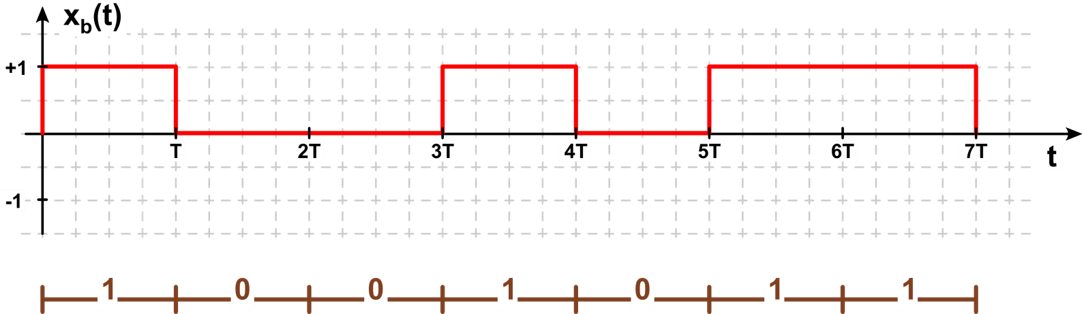
\includegraphics[width=8cm]{bilder/DigitaleBasisbandSignale/UnipolarNRZ.png}\newline
	\begin{itemize}[noitemsep]
		\item \textbf{Mark:} Amplitude A, \textbf{Space:} Amplitude 0
		\item \textbf{Aufwand (De-)Codierung:} sehr klein
		\item \textbf{Taktrückgewinnung:} ohne zusätzliche Codierung unsicher
		\item \textbf{DC-Freiheit:} sehr schlecht, viel DC-Anteil
		\item \textbf{Bandbreitenbedarf:} mittel
	\end{itemize}
	&
	\textbf{Bipolar NRZ-Signal}\newline
	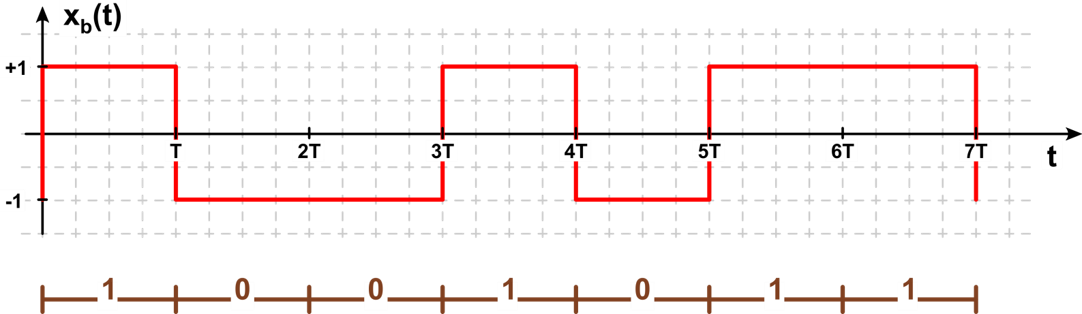
\includegraphics[width=8cm]{bilder/DigitaleBasisbandSignale/BipolarNRZ.png}\newline
	\begin{itemize}[noitemsep]
		\item \textbf{Mark:} Amplitude A, \textbf{Space:} Amplitude -A
		\item \textbf{Aufwand (De-)Codierung:} sehr klein
		\item \textbf{Taktrückgewinnung:} ohne zusätzliche Codierung unsicher
		\item \textbf{DC-Freiheit:} Abhängig vom Verhältnis von Mark und Space
		\item \textbf{Bandbreitenbedarf:} mittel (wie unipolares NRZ)
	\end{itemize}\\
	
	\hline
	
	\textbf{NRZ-Inverted-Signal (NRZI)}\newline
	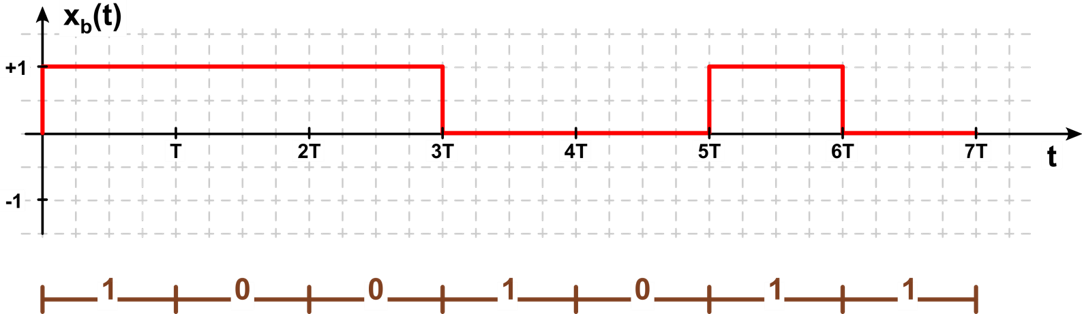
\includegraphics[width=8cm]{bilder/DigitaleBasisbandSignale/NRZInverted.png}\newline
	\begin{itemize}[noitemsep]
		\item \textbf{Bei NRZI, NRZ-M:} \textbf{Mark:} Amplitudenwechsel, \textbf{Space:} kein Amplitudenwechsel
		\item \textbf{Bei NRZ-S:} \textbf{Mark:} kein Amplitudenwechsel, \textbf{Space:} Amplitudenwechsel
		\item \textbf{Aufwand (De-)Codierung:} gering
		\item \textbf{Taktrückgewinnung:} ohne zusätzliche Codierung unsicher
		\item \textbf{DC-Freiheit:} sehr schlecht, viel DC-Anteil
		\item \textbf{Bandbreitenbedarf:} mittel
	\end{itemize}
	&
	\textbf{Unipolar RZ-Signal}\newline
	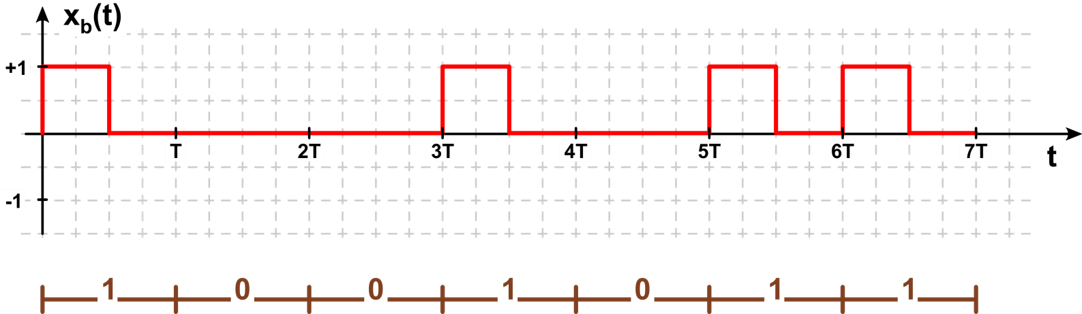
\includegraphics[width=8cm]{bilder/DigitaleBasisbandSignale/UnipolarRZ.png}\newline
	\begin{itemize}[noitemsep]
		\item \textbf{Mark:} Amplitude A (nach halber Bitzeit 0), \textbf{Space:} Amplitude 0
		\item \textbf{Aufwand (De-)Codierung:} gering
		\item \textbf{Taktrückgewinnung:} besser als NRZ, Space-Folgen immer noch heikel
		\item \textbf{DC-Freiheit:} sehr schlecht, viel DC-Anteil
		\item \textbf{Bandbreitenbedarf:} grösser als NRZ
	\end{itemize}\\
	
	\hline
	
	\textbf{Bipolares RZ-Signal}\newline
	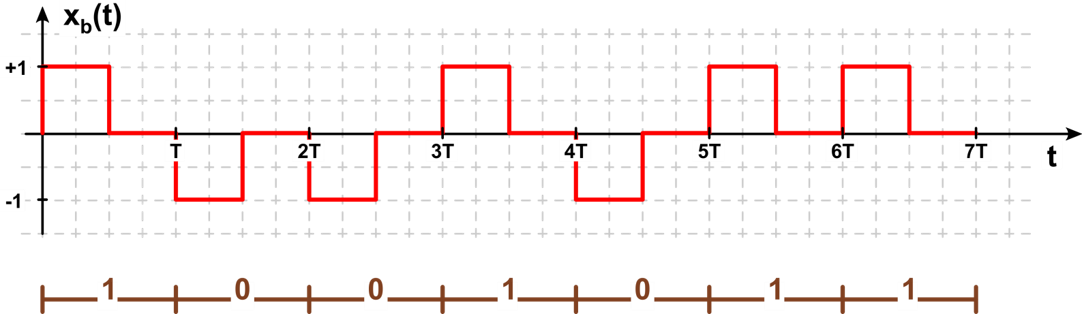
\includegraphics[width=8cm]{bilder/DigitaleBasisbandSignale/BipolarRZ.png}\newline
	\begin{itemize}[noitemsep]
		\item \textbf{Mark:} Amplitude A (nach halber Bitzeit 0), \textbf{Space:} Amplitude -A (nach halber Bitzeit 0)
		\item \textbf{Aufwand (De-)Codierung:} mittel
		\item \textbf{Taktrückgewinnung:} sehr gut
		\item \textbf{DC-Freiheit:} Abhängig vom Verhältnis von Mark und Space
		\item \textbf{Bandbreitenbedarf:} grösser als NRZ
		\item pseudoternäres Signal
	\end{itemize}
	&
	\textbf{Alternate Mark Inversion (AMI-NRZ, AMI-RZ)}\newline
	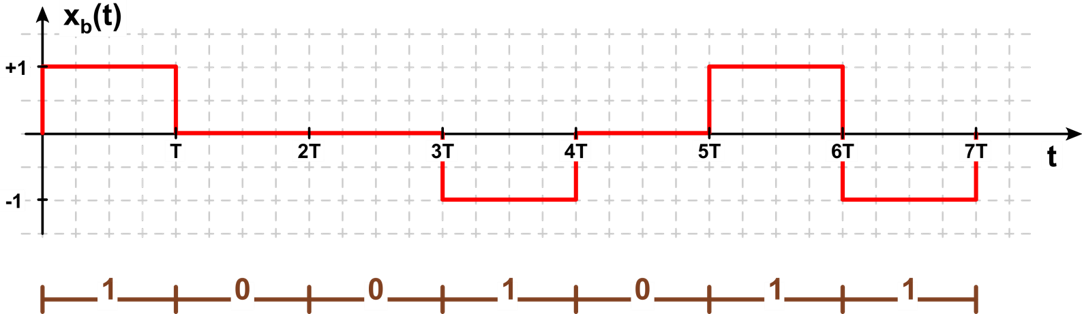
\includegraphics[width=8cm]{bilder/DigitaleBasisbandSignale/AMI.png}\newline
	\begin{itemize}[noitemsep]
		\item \textbf{Mark, Space:} Wie unipolares NRZ, doch mit alternierenden Amplituden $\pm$A für Mark
		\item \textbf{Aufwand (De-)Codierung:} mittel
		\item \textbf{Taktrückgewinnung:} besser als NRZ, Space-Folgen immer noch heikel
		\item \textbf{DC-Freiheit:} sehr gut
		\item \textbf{Bandbreitenbedarf:} sehr schlecht, viel DC-Anteil
		\item pseudoternäres Signal
	\end{itemize}\\
	
	\hline
	
	\textbf{Manchaster Code}\newline
	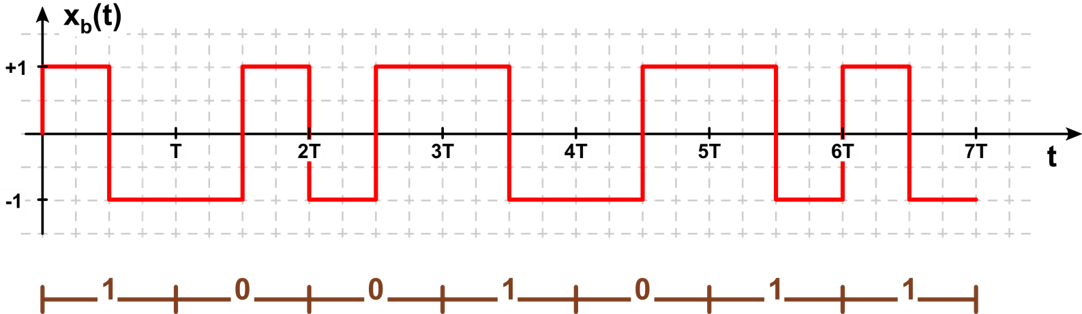
\includegraphics[width=8cm]{bilder/DigitaleBasisbandSignale/Manchaster.png}\newline
	\begin{itemize}[noitemsep]
		\item \textbf{Mark:} Übergang in Symbolmitte von +A nach -A, \textbf{Space:} Übergang in Symbolmitte von -A nach +A
		\item \textbf{Aufwand (De-)Codierung:} mittel
		\item \textbf{Taktrückgewinnung:} sehr gut
		\item \textbf{DC-Freiheit:} sehr gut
		\item \textbf{Bandbreitenbedarf:} grösser als NRZ
		\item pseudoternäres Signal
	\end{itemize}
	&
	\textbf{Multi-Level Transmit (MLT-3)}\newline
	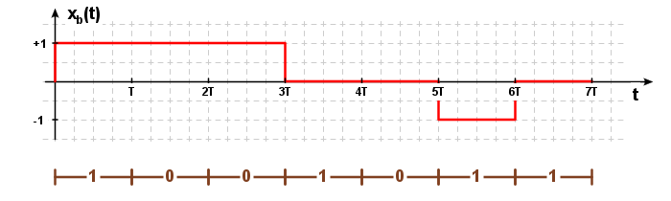
\includegraphics[width=8cm]{bilder/DigitaleBasisbandSignale/MultiLevelTransmit3.png}\newline
	\begin{itemize}[noitemsep]
		\item Pseudoternäres Signal mit 3 Amplitudenwerten +A, 0, -A (\textbf{Mark:} Amplitudenübergang, \textbf{Space:} konstante Amplitude)
		\item \textbf{Ablauf der Übergänge:} 0, +A, 0, -A, 0, +A, 0 etc.
		\item \textbf{Taktrückgewinnung:} heikel bei langen Space-Folgen
		\item \textbf{DC-Freiheit:} heikel bei langen Space-Folgen
		\item \textbf{Bandbreitenbedarf:} ca. halb so gross wie NRZ
	\end{itemize}\\
	
	\hline
	
	\textbf{Pulse Amplitude Modulation 5 (PAM-5)}\newline
	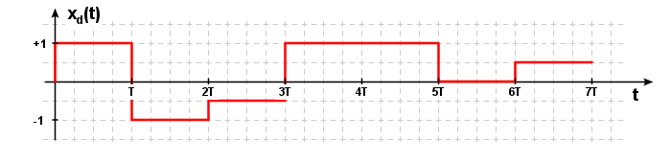
\includegraphics[width=8cm]{bilder/DigitaleBasisbandSignale/PulseAmplitudeModulation5.png}\newline
	\begin{itemize}[noitemsep]
		\item Mehrwertiges Signal mit fünf Amplitudenwerten: +A, +A/2, 0, -A/2, -A
		\item \textbf{Ablauf der Übergänge:} 0, +A, 0, -A, 0, +A, 0 etc.
		\item \textbf{Taktrückgewinnung:} heikel bei langen Space-Folgen
		\item \textbf{DC-Freiheit:} heikel bei langen Space-Folgen
		\item \textbf{Bandbreitenbedarf:} ca. halb so gross wie NRZ
	\end{itemize}
	&\\
	\hline
\end{longtable}

\newpage
\subsubsection{Pulse Shaping und ISI (Intersymbolic Interference) \schaum{101-5.13A}}
Da Übertragungskanäle in der Praxis keine idealen Eigenschaften 
(\textbf{limitierte Bandbreite}, Nichtlinearität, Verzerrungen) aufweisen,
werden die - von uns als rechteckig
angenommenen - Pulse verfälscht. Die Pulse werden \textbf{verbreitert} und \textbf{überlappen}
benachbarte Pulse, sodass beim Empfänger eine Unterscheidung der verschiedenen Symbole schwer
fällt. 
Das oben erwähnte Phänomen wird \textbf{intersymbolic interference} genannt.
Abhilfe schafft ein passendes Filter, welches dem Übertragungskanal vorgeschaltet wird. Das Filter
weist eine spezielle Impulsantwort auf, welche bei \textbf{gleichmässigen Zeitabständen} $T_s$
(Abtastzeiten) Null ist, ausser zum Zeitpunkt Null. Dadurch kann die ISI umgangen werden, wenn dann
genau zu diesen Zeiten abgetastet wird. \\ 

\textbf{Raised-Cosine Filter\schaum{103}} \\
Dieses Filter schafft Abhilfe bei ISI. Obwohl dies auch mit einem Idealen Filter
(Sinc-Frequenzgang) möglich wäre, wird ein Raised-Cosine mit folgenden Vorteilen eingesetzt:
\begin{itemize}
  \item Raised-Cosine-Puls fällt schneller ab als Sinc-Puls
  \item Raised-Cosine ist zwar auch akausal, aber in der Praxis einfacher realisierbar
  \item 1. Nyquist Kriterium wird von allen Raised-Cosine-Pulsen erfüllt
  \item 2. Nyquist Kriterium wird nur von Raised-Cosine-Puls mit $\alpha$ = 1 erfüllt
\end{itemize}

\begin{minipage}{9cm}
$$ f_B = \frac{1 + \alpha}{2 T_s} Hz \qquad \qquad \frac{1}{T_s} = \frac{2 f_B}{1 + \alpha}$$
$$ W = \frac{\omega_s}{2} = \frac{\pi}{T_s}$$
\end{minipage}
\begin{minipage}{9cm}
	$f_B$ benötigte Bandbreite, $[f_B] = Hz$ \\
	$\frac{1}{T}$ Pulsrate, $[\frac{1}{T}] = $ "Pulse pro Sekunde" \\
	$\alpha$ roll-off-Faktor, $[\alpha] = 1$ 
\end{minipage}
 
\[h(t) = \frac{1}{T_s} \cdot \left( \frac{\sin{W t}}{W t} \right) \left[ \frac{\cos{\alpha W t}}{1
- (2 \alpha W t / \pi)^2}\right]
\quad \laplace \quad
H(\omega) = \begin{cases}
	1 			
		&  	0 \leq | \omega | \leq (1-\alpha) W       \\
	\frac{1}{2} \left( 1 - \sin\left[ \frac{\pi}{2 \alpha W} (| \omega | - W)\right] \right)      
		&	(1-\alpha) W \leq | \omega | \leq (1+\alpha) W       \\
	0
		& 	| \omega | > (1+\alpha) W
            \end{cases}\]


\begin{center}  
		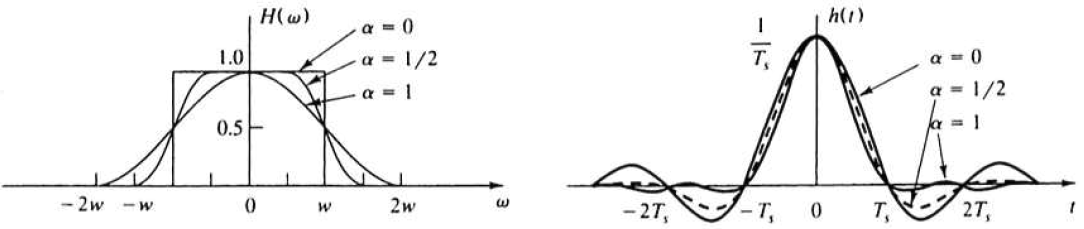
\includegraphics[height=3cm]{bilder/dig_raisedcosinefilter.png}
\end{center}

\subsubsection{1. Nyquistkriterium}
	\[h(n\cdot T_s-t_0) = 
		\begin{cases}
			h_0 & n= 0\\
			0 & n \neq 0
		\end{cases}
		\quad \laplace \quad
		\frac{1}{T_s} \cdot \sum\limits_{n = -\infty}^{+ \infty} H(\omega - n\frac{2\pi}{T_s}) = \underbrace{h_0}_{\text{Konstantes Spektrum}}
		\]
	Aus dem 1. Nyquistkriterium folgt die minimal benötigte Bandbreite um ISI zu verhindern: $B_{min} = 1/2 f_s$\\
	$\Rightarrow$ Dadurch wird das Augendiagramm bzgl. der Amplitude maximal geöffnet. \\
	$\Rightarrow$ Kein ISI beim Abtastzeitpunkt
	
\subsubsection{2. Nyquistkriterium}
	Zusätzlich zu den Nullstellen bei $n\cdot T_s$ (1. Nyquistkriterium) muss $h(t)$ auch an den Stellen $\pm 3/2 T_s$, $\pm 5/2T_s$, $\pm 7/2 T_s$, etc. eine Nullstelle aufweisen.\\
	$\Rightarrow$ So wird das Augendiagramm auch auf Zeitachse maximal geöffnet. \\
	$\Rightarrow$ Kein ISI beim Nulldurchgang

%TODO Augenmuster
\newpage
\subsubsection{Digitale Trägermodulation \schaum{104-5.14}}
Weil Binäre Nachrichtensignale selbst zu kleine Frequenzen aufweisen, sind sie nicht geeignet um
z.B. über den Äther zu schicken. Abhilfe schafft die binäre Trägermodulation.\\
Vorteile der Übertragung mit Trägersignal:
\begin{itemize}
	\setlength\itemsep{0.5pt}
	\item Physikalische Anpassung an Kanal (z.B. Funk)
	\item Mehrfache Nutzung des Kanals (Frequenzmultiplex)
	\item Erhöhung der Störfestigkeit der Übertragung
\end{itemize}

\begin{longtable}{|p{9cm}|p{9cm}|}
	\hline
	\textbf{Amplitude Shift Keying (ASK)}\newline
	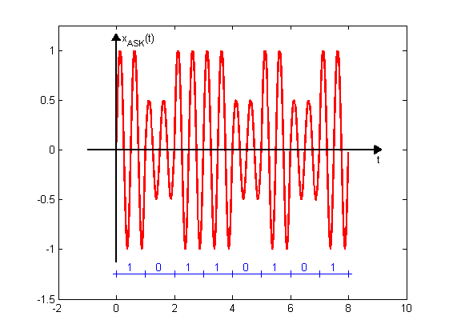
\includegraphics[width=8cm]{bilder/DigitaleTraegermodulation/ASK.png}
	\begin{itemize}[noitemsep]
		\item Trägeramplitude entspricht dem Wert des zu übertragenden Symbols (auch mehr als zwei Werte möglich)
		\item Binärer Fall: \textbf{Mark:} $A_c \cdot m(t) = A_1$, \newline \textbf{Space:} $A_c \cdot m(t) = A_0$
	\end{itemize}
	&
	\textbf{On-Off-Keying (OOK)}\newline
	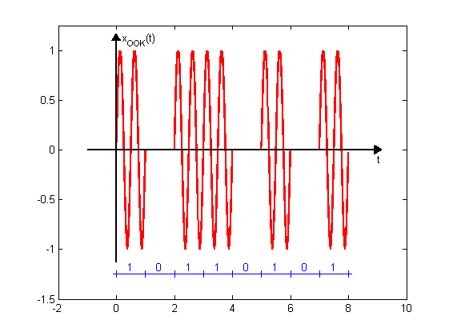
\includegraphics[width=8cm]{bilder/DigitaleTraegermodulation/OOK.png}
	\begin{itemize}[noitemsep]
		\item Binäre Variante von ASK: Amplitude vom Trägersignal wird durch Bitwerte ein- bzw. ausgeschaltet
		\item \textbf{Mark:} $A_c \cdot m(t) = A_1$, \textbf{Space:} $A_c \cdot m(t) = 0$
		\item vergleichbar mit unipolarem NRZ-Signal
	\end{itemize}\\
	
	\hline
	
	\textbf{Binary Phase Shift Keying (BPSK)}\newline
	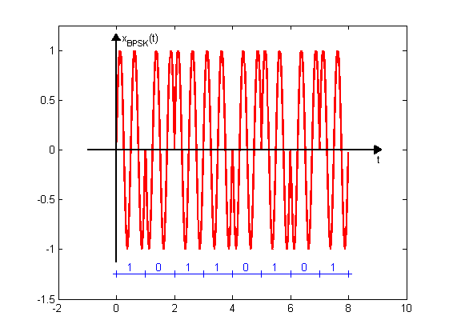
\includegraphics[width=8cm]{bilder/DigitaleTraegermodulation/BPSK.png}
	\begin{itemize}[noitemsep]
		\item Symbolwerte werden auf verschiedene Phasenlagen des Trägers abgebildet
		\item Binärer Fall: Phasenverschiebung des Trägers um 180\textdegree
		\item vergleichbar mit DSB-SC Modulation mit bipolarem NRZ-Signal
	\end{itemize}
	&
	\textbf{Differential BPSK (DBPSK)}\newline
	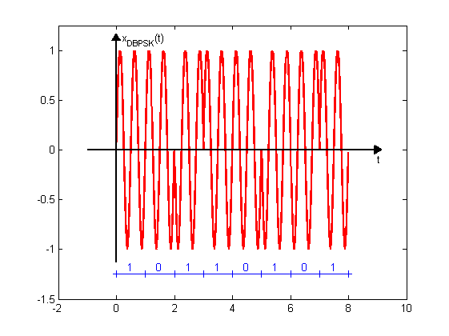
\includegraphics[width=8cm]{bilder/DigitaleTraegermodulation/DBPSK.png}
	\begin{itemize}[noitemsep]
		\item Problem bei BPSK: ohne zusätzliche Synchronisation sind Mark und Space nicht unterscheidbar
		\item Lösung von DBPSK: modulierendes Signal ist bipolares NRZ-I
		\item Nachteil: leicht höhere Fehlerrate
	\end{itemize}\\
	
	\hline
	
	\textbf{Frequency Shift Keying (FSK)}\newline
	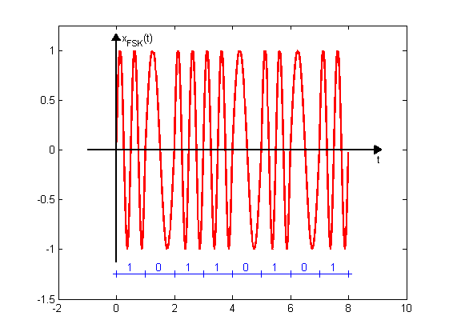
\includegraphics[width=8cm]{bilder/DigitaleTraegermodulation/FSK.png}
	\begin{itemize}[noitemsep]
		\item Jeder Symbolwert erzeugt eigene Trägerfrequenz
		\item Wenn Phasensprünge erlaubt: FSK kann durch Kombination mehrerer OOK-Signale gebildet werden
		\item keine Phasensprünge (continuous phase modulation): mit NRZ moduliertes FM-Signal (Vorteil: kleinere Bandbreite)
	\end{itemize}
	&
	\textbf{Minimum Shift Keying (MSK)}\newline
	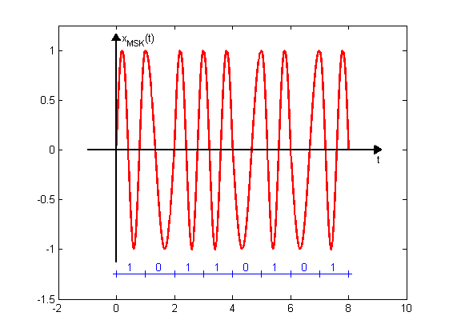
\includegraphics[width=8cm]{bilder/DigitaleTraegermodulation/MSK.png}
	\begin{itemize}[noitemsep]
		\item Binäre continuous phase FSK, bei welcher die über die Symbolzeit integrierte Phasenabweichung gegenüber dem nicht-modulierten Träger $\pm \pi/2$ beträgt
		\item Vorteil zu continuous phase FSK: Signale für Mark und Space sind zueinander orthogonal, womit die Bitfehlerrate beim Empfänger reduziert werden kann
	\end{itemize}\\
	
	\hline
\end{longtable}

\subsubsection{mehrwertige Signale}
\begin{multicols}{2}
    \begin{center}
	QAM-16\\
	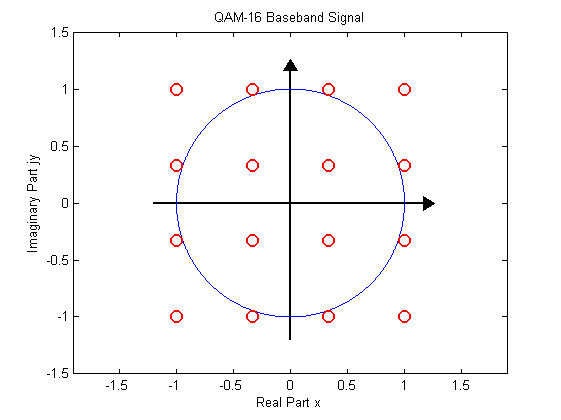
\includegraphics[width=6cm]{bilder/qam_16.png}\\
	\end{center}
	Amplituden und Winkel ändern sich.
	Die Amplituden sind mit trigo zu berechnen:
	$\textcolor{green}{\sqrt{2}}; \textcolor{red}{\frac{\sqrt{10}}{3}}; \textcolor{blue}{\frac{\sqrt{2}}{3}}$
	\columnbreak

    \begin{center}
	PSK-8\\
	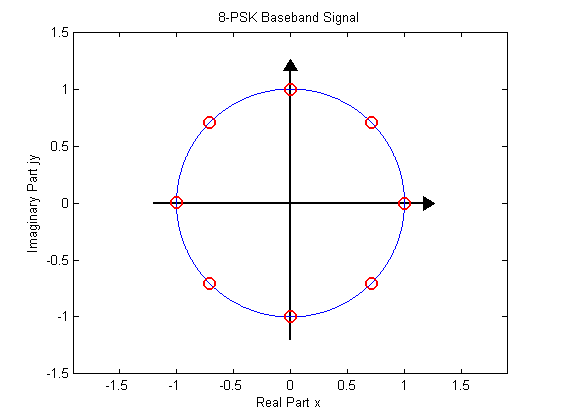
\includegraphics[width=6cm]{bilder/psk_8.png}\\
	Amplituden sind konstant nur Winkel ändern sich.\\
	Es gilt: $B_{PSK} = 2\cdot B_m$
	\end{center} 

\end{multicols}
	Anzahl bits pro Symbol: $log_2\left(n\right)$\\
	z.B. 8-PSK oder 8-QAM $= log_2(8) = 3 \frac{Bit}{Symbol}$\\
	Frequenzverhalten wie anloge Gegenstücke.
